\documentclass[a4paper, twocolumn]{article}

\usepackage[margin=1in]{geometry}    
\usepackage[english]{babel}
\usepackage[utf8]{inputenc}
\usepackage[noend]{algpseudocode}
\usepackage[title, page]{appendix}
\usepackage[backend=biber,style=numeric,sorting=ynt]{biblatex}
\usepackage{titlesec}
\usepackage{hyperref}
\usepackage{fancyhdr}
\usepackage{algorithm}
\usepackage{arevmath}
\usepackage{mathtools}   
\usepackage{graphicx}
\usepackage{comment}
\usepackage{float}
\usepackage{tabularx}

\addbibresource{biblio.txt}
\graphicspath{ {./Figures/} }  
\titleformat{\section}[block]{\filcenter}{\thesection}{1em}{}
\titleformat{\subsection}[block]{\slshape}{\thesubsection}{1em}{}
\renewcommand{\thesection}{\Roman{section}} 
\renewcommand{\thesubsection}{\thesection.\Roman{subsection}}

%opening
\title{Transient Terminal Set GP: A New Approach to Improving Interpretability in Symbolic Regression Models}
\author{Asher Stout}
\begin{document}
\maketitle
\begin{abstract}
Symbolic Regression (SR) models generated using Genetic Programming have the potential to be composed of hundreds of feature inputs representing advanced non-linear relationships. Such models prove difficult to interpret without advanced domain knowledge and the use of post-hoc interpretability techniques such as ELA can only approximate these models. Generating SR models with lower tree sizes is a prerequisite for improving model interpretability, however modern multi-objective GP methods often have drawbacks in the form of a trade-off between model accuracy and interpretability. Transient Terminal Set GP (TTSGP) is a new GP algorithm which aims to reduce the tree sizes of evolved SR models without reducing accuracy, while simultaneously broadening the range of solutions produced and streamlining the evolutionary search process. This is achieved through tracking the improvements made in candidate solutions across generations and inserting subtrees which caused a significant improvement in fitness into the population during a genetic operation called Transient Mutation. Experiments show that TTSGP has the potential to improve the interpretability of SR models when compared with MOGP, however such advancements are inconsistent across datasets and do not necessarily improve the diversity of solutions and the evolutionary search process.
\end{abstract}

\section{Introduction}
In recent years Artificial Intelligence has experienced a rapid rise in interest in data-critical settings, most notably in the finance and healthcare sectors. As the prevalence of AI in the working world continues to expand, so does the need for its models to be understandable to an audience with limited or no exposure to AI and Machine Learning concepts. Regression problems present an additional challenge in that ideal solutions may rely on hundreds or thousands of feature variables and may represent advanced non-linear relationships. Such models are incomprehensible to humans but may yet be required in their unaltered forms for domain-specific tasks. Interpretability is fast becoming as indispensable as accuracy in today's AI applications.

Several methods to improve the interpretability of symbolic regression (SR) models have been proposed in recent years, with numerous success stories for both post-hoc explanation techniques and in-model optimizations. Filho et al propose Explanation by Local Approximation (ELA), a post-hoc technique which seeks to explain a single prediction made by a model by computing the importance of each input feature\cite{1}. By aggregating the input feature importances at each data point using ELA, a global feature ranking is produced which shows a strong approximation with the original SR model yet is significantly more interpretable.

Multi-objective Genetic Programming (GP) has been another area of recent scholarship which has produced exciting results for generating interpretable SR models. Kommenda et al define an adapted NSGA-II algorithm which utilizes a Pareto-optimal front to breed with the population and alter the domination strategy itself to reduce the prevalence of single-node solutions\cite{2}. This approach has been proven during experimentation to improve the interpretability of SR models, yet remains susceptible to noisy data and can fail to converge to the accuracy achieved by single-objective GP models.

A new multi-objective GP approach is proposed in this report which intends to further improve the interpretability of SR models, dubbed the Transient Terminal Set. The Transient Terminal Set aims to improve SR model interpretability by identifying the subtrees in a population which generated the greatest improvements to fitness and distributing these subtrees as terminals used during a third genetic operation called Transient Mutation. This process is hoped to improve the search process for optimal solutions, enabling faster convergence and the potential for a greater range of solutions within the Pareto front.

\section{Previous Research in Interpretable AI}

Genetic programming has been utilized in a multitude of capacities for improving model interpretability. Single objective GP and multi-objective GP have both seen substantial developments within this area of research via a variety of techniques, ranging from feature construction and post-hoc interpretability to new GP algorithms.

Single-objective GP has mainly been applied in the former two categories. Ferreira et al have proposed a post-hoc local explainer for AI models called Genetic Programming Explainer (GPX)\cite{4}. GPX generates a set of points surrounding a model prediction and generates a function using GP to approximate the local relationship at that prediction. Experimentation with this technique demonstrated it generates interpretable expressions which greatly improve the interpretability of models generated by black-box techniques like Neural Networks and SVMs. GPX is limited by its scope, which requires a local approximation to be constructed for each prediction, and may thus not be as suited to problems which require interpretable global solutions.

Multi-objective techniques have meanwhile been more abundant and applicable in trying to solve the interpretability problem and have produced major advancements in recent scholarship. Icke et al defined Multi-objective GP projection pursuit (MOG3P), a method which aims to improve the visual interpretability of classification problems\cite{3}. Under MOG3P, feature extraction is performed to evolve features which when projected into a 2D space are more visually and semantically interpretable than models using the original feature set. Experiments proved MOG3P can obtain data representations for classification problems better than those obtained by similar methods, like principal component analysis and multiple discriminant analysis. However this method is unproven for regression problems, and may only exacerbate interpretability issues if used in a context where maintaining the original feature set is desired.

Chen et al utilize multi-objective GP to construct hybrid SR models\cite{5}. Hybrid SR models are composed of multiple sub-functions encoded using improved expression trees (IET), where each node is representative of a terminal or subfunction and has an associated multiplier. Thus, both the SR models and its components are jointly optimized using multi-objective GP, which potentially allows for candidate solutions to be produced which are more interpretable. Experimentation demonstrated this method makes significant improvements to both accuracy and interpretability compared with other techniques such as SVR and XGBoost. This method represents one of the most significant advancement to interpretable SR utilizing multi-objective GP authored in recent years, though itself is heavily dependent on IET encoding, which itself requires further research.

\section{Transient Terminal Set GP}
The Transient Terminal Set seeks to improve the interpretability of Symbolic Regression models by tracking evolutionary improvements in the population across generations. When a candidate solution undergoes either regular crossover or mutation, the trans-generational fitness change is calculated. Should this reflect a Pareto improvement in the fitness values and result in a significant improvement in at least one fitness value (\textit{solution accuracy} or \textit{solution complexity}) the altered subtree of the candidate solution is added to the Transient Terminal Set.

These subtrees are then distributed among the population via a third genetic operator, Transient Mutation. When a member of the population undergoes Transient Mutation, a randomly-selected subtree is replaced with a member of the Transient Terminal Set. Thus, the Transient Terminal Set distributes proven subtrees that result in Pareto improvements to fitness throughout the population. It is theorized that this genetic operation can result in candidate solutions with significantly improved accuracy and complexity measures over the course of evolution, thereby allowing for a greater diversity of optimal solutions and faster convergence. Thus, the Transient Terminal Set represents a marked improvement over the entirely randomized mutation of standard multi-objective GP. 

Transient Terminal Set GP (TTSGP) is described using pseudocode in Algorithm 1, and its Python implementation is accessible via GitHub\footnote[1]{\url{https://github.com/VeryEager/transient-terminal-gp}}. The three parameters TTSGP introduces to GP require further explanation in order to understand their purposes and implications. These were named the transient mutation probability, subtree lifespan, and subtree threshold.

Not dissimilar to crossover and mutation, the rate at which Transient Mutation is applied to the population is controlled by the \textit{transient mutation probability} (tmutpb). During evolution it is still expected that $CXPB + MUTPB + TMUTPB = 1.0$.

The \textit{subtree lifespan} controls the number of generations valid subtrees remain in the Transient Terminal Set for. Lower values indicate an expectation for numerous short-lived improvements in fitness over a short duration, while higher values imply gradual improvements are made over an extended period. This is best illustrated using an evolution's current generation; initial generations see a variety of candidate solutions improve significantly as they approximate to local optimums. Meanwhile, later generations see fewer significant changes in fitness as candidate solutions converge on a singular global optimum. During experimentation this parameter was left at \textbf{5}.

Finally, the \textit{subtree threshold} quantifies the change in candidate solution fitness which is considered significant enough to warrant the inclusion of its changed subtree in the Transient Terminal Set. In practice, the change in a candidate solution's fitness is calculated as a percent. Should either its percentage improvement in accuracy or complexity be above the subtree threshold (calculated as the percentage at the \textit{N}the percentile using the population)then the corresponding subtree is added to the Transient Terminal Set.
\begin{algorithm*}[h]
	\caption{Multi-objective GP using the Transient Terminal Set (TTSGP)}
	\hspace*{\algorithmicindent} \textbf{Input:} population size \(\rho\), crossover probability \textit{p$_{c}$}, mutation probability \textit{p$_{m}$}, transient mutation probability \textit{p$_{d}$}, terminal set \(T\), function set \(F\), lifespan \(\alpha\) \\
	\hspace*{\algorithmicindent} \textbf{Define:} generation \(G_{n}\), individual fitness \(f_{i}\), transient terminal set \(M_{G_{n}}\), subtree threshold \(f_{t, G_{n}}\) \\ 
	\begin{algorithmic}[1]
		\State Initialize starting population \textit{$ P_{G_{0}} $}, \(M_{G_{0}}\leftarrow \emptyset\), \(f_{t, G_{0}} \leftarrow 0\)
		\While{\textit{no improvement in} \(\max f_{i}\in P_{G_{n}}\) \textit{since} \(P_{G_{n-5}}\)} \Comment{Evolve generation  \(G_{n+1}\)}
		\State \(P_{G_{n+1}}\leftarrow \emptyset\), \(M_{G_{n+1}}\leftarrow M_{G_{n}}\)
		\While{len\(P_{G_{n+1}} \neq \rho\)}	\Comment{Update population \(P_{G_{n+1}}\)}
		\State Perform crossover $\forall i\in P_{G_{n}}$ with \textit{p$_{c}$}
		\State Perform mutation $\forall i\in P_{G_{n}}$ with \textit{p$_{m}$}, \(T\), \(F\)
		\State Perform transient mutation $\forall i\in P_{G_{n}}$ with \textit{p$_{d}$, \(M_{G_{n}}\)}
		\State $P_{G_{n+1}} \leftarrow P_{G_{n+1}}\cup \{i | i_{offspring}\}$
		\EndWhile\newline
		\ForAll{subtree \(s \in  M_{G_{n+1}}\)}	\Comment{Update transient terminal set \(M_{G_{n+1}}\)}
		\If{\(age(s) > \alpha\)}
		\State Prune \(s\) from \(M_{G_{n+1}}\)
		\EndIf
		\EndFor
		\State Compute $f_{t, G_{n}}$ from $\forall f_{i} \in P_{G_{n+1}}$
		\For{$i\in P_{G_{n+1}}$}	
		\State $f_{c}\leftarrow \Delta f_{i}$ from \(G_{n}\) to \(G_{n+1}\)
		\If{ $f_{c} > $ \(f_{t, G_{n}}\)}
		\State \(M_{G_{n+1}} \leftarrow M_{G_{n+1}} \cup \{\)subtree \(s\in i \}\)
		\EndIf
		\EndFor 
		\EndWhile
	\end{algorithmic}
\end{algorithm*}

\section{Experiment Methodology}
\subsection{Experiment Design}
Several experiments were performed to definitively determine whether TTSGP exhibits any improvement in the interpretability of SR models over other modern methods. The experiments consisted of recording the fitnesses of Symbolic Regression trees for TTSGP and several benchmark GP methods at each generation in their evolutions across several regression datasets. For the purposes of the experiments, the accuracy and complexity of a Symbolic Regression tree were defined as the RMSE over the test set and the candidate solution's tree size, respectively. 

The GP methods used during experiments consisted of Single-objective GP (SOGP), Single-objective TTSGP (SOTTGP), Multi-objective GP and TTSGP with 50 generations and population size of 500, Multi-objective GP and TTSGP with 250 generations and population size of 200, and TTSGP with optimal parameter settings (see \textit{IV.III}). All methods were written using Python's DEAP library. The Multi-objective methods and TTSGP utilized the NSGA-II algorithm for optimization. The regression datasets were split into 70\% training instances and 30\% testing instances prior to evolution. Results for the GP methods were averaged across 50 seeds on each dataset. The evolutionary parameters for the experiments are summarized in Table M.
\begin{table}[h]
	\begin{center}
		\caption{Evaluation Experiments' Settings}
		\label{table:M}
		\begin{tabularx}{\columnwidth}{>{\hsize=1.5\hsize}X|>{\hsize=.5\hsize}X}
			\hline
			Generations&50 or 250\\
			Population Size&200 or 500\\
			CXPB&0.8\\
			MUTPB&0.1\\
			TMUTPB&0.1\\
			Subtree Threshold&90\\
		\end{tabularx}
	\end{center}
\end{table}
\subsection{Datasets}
Four common regression datasets were selected for the experiments, and are presented and summarized in Table N. They provide a range of distributions and non-linear relationships for identification in the GP methods.
\begin{table}[h]
	\begin{center}
		\caption{Dataset Information}
		\label{table:N}
		\begin{tabularx}{\columnwidth}{>{\hsize=1.5\hsize}X|>{\hsize=.25\hsize}X|>{\hsize=.25\hsize}X}
			Dataset&Size&Features\\
			\hline
			Red Wine Quality&1599&11\\
			White Wine Quality&4898&11\\
			Boston House Price&506&13\\
			Concrete Compressive Strength&1030&8\\
		\end{tabularx}
	\end{center}
\end{table}

None of the selected datasets were preprocessed except to remove non-numeric or constant features from the data, and are readily available at the UCI Machine Learning Repository\footnote[2]{\url{https://archive.ics.uci.edu/ml/index.php}}. The preprocessed versions used for these experiments remain accessible via the aforementioned GitHub repository\footnote[3]{\url{https://github.com/VeryEager/transient-terminal-gp}}.
\subsection{TMUTPB \& Subtree Threshold Experiments}
In addition to the aforementioned experiments, two additional experiments were performed using TTSGP to determine the optimal TMUTPB and subtree threshold values. The optimal value of these parameters was defined as the value within the ranges [0.05, 0.9] and [5, 100] with step sizes of (0.05, 5) which resulted in equal or lower RMSE than other parameter values while providing the most significant reduction in tree size at the final generation. To ensure the probabilities of the genetic operators did not sum to a value $>$ 1.0 during the TMUTPB experiment, the CXPB was inversely correlated with the TMUTPB value according to the formula $0.9-TMUTPB$.

The Red Wine Quality dataset was utilized to evaluate the performance of TTSGP at each parameter value. As with the previous experiments, the evolutionary results for each parameter value were averaged across 50 seeds. The identified optimal parameter values were then used during the evaluation of the performance of TTSGP in the original experiments (see \textit{IV.I}). Table O summarizes the evolutionary parameters for the TMUTPB and Subtree Threshold experiments.
\begin{table}[h]
	\begin{center}
		\caption{TMUTPB \& Subtree Threshold Experiment Settings}
		\label{table:O}
		\begin{tabularx}{\columnwidth}{>{\hsize=1.5\hsize}X|>{\hsize=.5\hsize}X}
			\hline
			Generations&50\\
			Population Size&500\\
			CXPB (threshold experiment)&0.8\\
			MUTPB&0.1\\
			TMUTPB&[0.05, 0.9]\\
			Subtree Threshold&[5, 100]\\
		\end{tabularx}
	\end{center}
\end{table}

\section{Results \& Discussion}
\subsection{Parameter Experiments}
The results presented in Table Y and Table Z display the highest-accuracy SR model at the 50th generation of evolution averaged across 50 seeds for each parameter value presented. As discussed in IV.III, the purpose of these experiments were to determine the optimal transient mutation probability and subtree threshold values for use in TTSGP. An optimal value was defined in IV.III as a value which resulted in equal or lower RMSE than other parameter values while providing the most significant reduction in tree size. 

Using these constraints during analysis, the results in Table Y and Table Z do not indicate there is a singular optimal parameter value for either TMUTPB and the subtree threshold. There is no one such parameter value which simultaneously achieves the lowest RMSE and tree size. However, there were values for both parameters which resulted in significantly lower tree sizes while achieving approximately equal accuracy to nearby values. The identified parameter values were subtree threshold = \textbf{85th percentile} and transient mutation probability = \textbf{0.15}. Note that Table Y and Table Z are centered around the neighborhood of these points. 

These parameter values approximate the accuracy of nearby solutions while achieving the minimum tree size in their respective experiments. A subtree threshold of 85 (Table Y) achieves an RMSE within a margin of 0.015 from the highest recorded value (located at a threshold of 100 and with a RMSE/tree size tuple of (0.771, 12.48)), while reducing the tree size by an average 0.44 nodes from the next smallest complexity at the 90th percentile threshold. This suggests there is a trade-off between candidate solution accuracy \& complexity when utilizing TTSGP. 

This inverse relationship is prevalent in the results for the optimal TMUTPB value of 0.15 (Table Z), which is approximately 0.42 RMSE worse than the lowest recorded RMSE of 0.744 at a TMUTPB of 0.75. Yet this TMUTPB value improves the complexity of candidate solutions by an average of 1.48 nodes when compared with the second-smallest tree size of 8.4 located at a TMUTPB of 0.1. Due to the general ability of these parameter values to reduce tree size while approximating model RMSE, a TMUTPB = 0.15 and subtree threshold = 85 were used as the 'optimal' parameter values during the evaluation experiments.

In addition to the identified optimal parameter values, the results for 'unoptimal' parameter values provide fascinating insights into the implications of the TTSGP algorithm. One such pattern which emerged in the TMUTPB results was the tendency for lower transient mutation probabilities to produce candidate solutions with smaller tree sizes. Transient mutation values within the range [0.05, 0.25] produced candidate solutions with tree sizes under 10, with the minimum centered at 0.15. TMUTPB values over 0.25 resulted in progressively larger tree sizes, with the maximum value of 13.52 at a TMUTPB of 0.75, though these larger trees generally improved the RMSE of candidate solutions by an average of 0.024. Once the TMUTPB reached 0.9 (and thus entirely replaced crossover with transient mutation) the tree size spiked to an average of 22.56, though RMSE was not affected. Transient Mutation demonstrates similarities with standard GP mutation in that it does not necessarily distribute genetic information efficiently throughout the population; crossover should still be used as the primary means for evolving high-fitness candidate solutions. Transient Mutation should act in a capacity which further refines existing individuals and should therefore have a low probability of occurring relative to crossover.

Meanwhile, the subtree threshold experiment results indicate TTSGP may negatively affect the diversity of populations when the subtree threshold is considerably low. When the subtree threshold was set at a value in the range of [5, 65] the results were identical, with an RMSE/tree size tuple of (0.781, 8.56). This unusual pattern likely occurs due to the functionality of the Transient Terminal Set as a set; that is, disallowing the inclusion of identical subtrees. At lower threshold values, all possible subtrees which result in improved fitness are already present in the set, so the population converges on a local optimum while its members undergo transient mutation until they are homogeneous. At that point no further improvements in fitness can be made with the existing genetic operators. At subtree threshold values above 65 some subtrees are presumably absent from the set, meaning Transient Mutation is not applied as frequently with similar subtrees early during an evolution, thereby reducing its homogeneity and allowing for a greater range of candidate solutions. It is imperative, therefore, that the subtree threshold value be strictly controlled to only allow for substantial improvements in fitness to be considered and should typically be above the value of 65, though this is ultimately dependent on the dataset used.
\newline
\begin{table}[H]
	\begin{center}
		\caption{Threshold Experiment Results (RMSE, tree size)}
		\label{table:Y}
		\begin{tabularx}{\columnwidth}{X|X}
			Threshold&Fitness\\
			\hline
			5&(0.781, 8.56)\\
			...&...\\
			60&(0.781, 8.56)\\
			65&(0.783, 8.76)\\
			70&(0.776, 8.4)\\
			75&(0.784, 10.52)\\
			80&(0.777, 10.92)\\
			\textbf{85}&\textbf{(0.786, 7.96)}\\
			90&(0.780, 8.4)\\
			95&(0.778, 8.56)\\
			100&(0.772, 12.48)\\
		\end{tabularx}
	\end{center}
	\begin{center}
		\caption{TMUTPB Experiment Results (RMSE, tree size)}
		\label{table:Z}
		\begin{tabularx}{\columnwidth}{X|X}
			TMUTPB&Fitness\\
			\hline
			0.05&(0.783, 9.84)\\
			0.10&(0.780, 8.4)\\
			\textbf{0.15}&\textbf{(0.786, 6.92)}\\
			0.20&(0.761, 9.36)\\
			0.25&(0.769, 9.52)\\
		\end{tabularx}
	\end{center}
\end{table}

\subsection{Interpretation \& Discussion}
The evaluation experiments tracked four key variables reported by the methods during evolution; the fitness of the best (highest-RMSE) candidate solution on both the training and testing data, the fitness of the most balanced (candidate solution closest to the 'ideal' model of (0.0, 0)) solution on the testing data, and the average execution time of the method. The fitnesses reported in the first three tables were recorded at the final generation and were averaged across 50 seeds. These results are reported in their raw forms in Appendix A, while the evolutions of the best models generated by each method are presented in Figures 1-16 in Appendix B.

It is immediately apparent in the results for the testing fitness (Table 6) that TTSGP methods do not necessarily result in reduced tree sizes for the best individual. MOGP with 50 generations and a population size of 500 achieved the best RMSE score of all multi-objective methods in 3 of the 4 datasets; in the Red Wine Quality data it tied with TTSGP with the same evolutionary parameters. Of TTSGP methods, TTSGP with 50 generations and a population size of 500 achieved the best RMSE performance across all datasets, though other TTSGP methods were within $\tilde{}$6.9\% RMSE on average. A safe assertion can be made that TTSGP methods are competitive among themselves in terms of the RMSE, though a different conclusion can be drawn when comparing tree sizes. 

TTSGP methods achieved the smallest tree size in three of the four datasets, while MOGP with 50 generations and a population size of 500 achieved the lowest in only the White Wine data. Of the TTSGP methods, TTSGP with optimal parameters, 250 generations and a population size of 200 consistently produced tree sizes lower than other TTSGP methods (aside from one outlier in the Concrete Strength data). On average, TTSGP methods typically reduced the tree size of candidate solutions by 0.5 to 1.5 nodes, indicating an improvement to model interpretability is possible. As previously discussed however, this improvement is marred by the consistently higher RMSEs of all TTSGP methods when compared with MOGP alternatives. Despite producing models with the lowest tree sizes, TTSGP with optimal parameters, 250 generations and a population size of 200 performed the worst in terms of RMSE across all datasets. Based on the performance of TTSGP methods when they are compared with MOGP alternatives, we can summarize that some TTSGP methods typically produce SR models with reduced tree sizes - at the expense of RMSE.

Surprisingly, TTSGP with the optimal parameter values and the same evolutionary parameters as the aforementioned methods performed identical to TTSGP with 50 generations and a population size of 500 across all datasets. This behavior is exceedingly unnatural though does not itself indicate that the parameter values have no effect on evolution, as is evidenced by the results for TTSGP with 250 generations and a population size of 200 being different from the same TTSGP experiment with optimal parameter values. While unlikely, it is possible that altering the subtree threshold did not change results due to the distribution of model improvements during evolution being skewed towards 0 (or even negative). However this does not exonerate the inability of the changed TMUTPB value to improve candidate solutions. An analysis of the experimentation code discovered no errors or issues which could have potentially led to this behavior, and further research must be undertaken to discern the underlying cause.

A final point on the results for the single-objective methods can be made from Table 6. As expected, both SOGP and SOTTGP achieved RMSE significantly lower than the multi-objective methods, though at the cost of tree size (which were exponentially larger than even the largest tree sizes from the multi-objective methods). Interestingly, SOTTGP achieved a higher RMSE than SOGP in 3 of the 4 datasets, with the improvement made reaching a maximum of 8.1\% in the Concrete Strength data. This suggests the inclusion of the Transient Terminal Set in GP does have the potential to improve the fitness of candidate solutions, at least within one-dimensional optimization problems.

Results for the training fitness of the best candidate solution (Table 7) are not dissimilar to the RMSE values reported in the testing fitness (Table 6). All methods tended to overfit slightly on the training data, with the difference between the training and testing RMSE often in the fractions of a percent for both TTSGP and MOGP. TTSGP methods appear to be equally as robust to overfitting as MOGP methods.

In addition to the testing accuracy of the best candidate solution, the testing fitness of the most balanced candidate solution from the evolution was also recorded (Table 8). This metric provides insight into the relative distribution of candidate solutions across the Pareto front. As explained in I, the Transient Terminal Set aims to expand the range of possible solutions within the Pareto front, and thus the most balanced candidate solution would likely see a significant difference in RMSE/tree size from the best candidate solution than in MOGP methods. The results corroborate the conclusions drawn from the results on the best candidate solutions, though do not indicate TTSGP evolved more 'balanced' models than MOGP methods.

As with the results of the best candidate solutions, the fitness of the balanced candidate solutions reflect the tendency for TTSGP methods to reduce tree size while sacrificing RMSE, however the inverse relationship is here more pronounced. All TTSGP methods achieved tree sizes 0.75 nodes smaller than MOGP methods on average across the four datasets but are unable to approximate the accuracy achieved by MOGP with 50 generations and a populations size of 500 (which returned the highest RMSE of all tested methods across the four datasets). On average, TTSGP methods achieved RMSEs approximately $\tilde{}$13.1\% lower than MOGP, though the variance across datasets was substantially more pronounced, for example in the Concrete Strength data. Compared to the average difference of $\tilde{}$6.9\% between MOGP and TTSGP methods in the results for the best candidate solutions, a further reduction in tree size (around the maximum of 1.5 nodes recorded in the results for the best candidate solutions) would need to be present in the results for the balanced candidate solutions to quantify as an improvement. In summary, the balanced models generated by TTSGP do not necessarily show any improvement in interpretability compared to MOGP methods, and further exacerbate the shortcomings of the Transient Terminal Set. 

A brief discussion of the execution times of the methods is also warranted (Table 9). TTSGP methods using the same evolutionary parameters as their MOGP counterparts evolved a single seed approximately 50\% slower in most cases. The relationship between execution times is most pronounced in the results for TTSGP with 250 generations and a population size of 200. The execution time for the MOGP methods follows an approximately linear relationship, with twice as long being required for the latter due to double the number of genetic operations being undertaken. TTSGP does not share this relationship; a non-liner, potentially exponential relationship exists which results in TTSGP with 250 generations and a population size of 200 taking up to 5 times as long to evolve as TTSGP with 50 generations and a population size of 500. In some datasets such TTSGP methods even perform worse than their single-objective counterparts.

Figures 1 through 16 presented in Appnedix B provide key insights into the effects of TTSGP on the evolution of candidate solutions, particularly in the convergence of candidate solutions to the global optimum. One of the theorized improvements of TTSGP identified in I was the possibility for convergence to global optimums to be achieved in fewer generations than existing MOGP and single-objective methods. The patterns and irregularities present in the Figures provide evidence both for and against this theory.

An evaluation of the evolutions for SOGP and SOTTGP suggest the Transient Terminal Set is able to achieve RMSEs comparable to SOGP in fewer generations. SOTTGP reaches SOGP's RMSE values in 10 less generations on average within the training data. The results over the test set contain irregularities for both techniques in the form of spikes in the RMSE value over a short number of generations. These spikes are of both greater magnitude and duration in SOTTGP though do not have any long-run effect on evolution in 3 of the 4 datasets (in the case of the Boston House Price data, it remains possible were the evolution extended by several generations SOTTGP would again return to an RMSE lower than SOGP, as is the case in the training data).

TTSGP performs exceedingly similarly to MOGP in its training RMSE across all experiments, and does not directly support the theory of the Transient Terminal Set improving evolution speed. In most experiments TTSGP methods were on par or slightly worse than MOGP methods, though performed considerably worse in the Concrete Strength and Boston House Price datasets, where they failed to converge to the RMSE obtained by MOGP. The inability of TTSGP to converge to MOGP is reflected in the RMSE trajectories across the test set, which all closely mimic the training data. There was no significant difference in the evolution of the tree sizes for the candidate solutions across TTSGP and MOGP methods; both techniques tend to gradually increase tree size as the evolution progresses, though not to the extent of the single-objective techniques.

The conclusions drawn from the full suite of results obtained from the experiments, including both the raw results in Appendix A and the evolutionary figures presented in Appendix B, are that the addition of the Transient Terminal Set in GP occasionally reduces the tree size of the best candidate solutions at the cost of higher RMSE values. There is only limited evidence for TTSGP improving the diversity of the Pareto front candidate solutions and allowing for faster convergence during the evolutionary search process.

\subsection{Statistical Significance Tests}
Statistical significance tests on the distribution of best solutions at the final generation of evolution were performed to authenticate or disprove the conclusions drawn in V.II. These significance tests took the form of one-sided Mann-Whitney U tests and compared all methods against MOGP with 50 generations and a population size of 500, as this was the method which was considered the standard of all multi-objective methods. 

The null hypothesis was that the distribution of results for the tested method had the same (or greater) distribution than MOGP with 50 generations and a population size of 500. The alternative hypothesis was that the distribution of results for the tested method had a lower distribution than MOGP with 50 generations and a population size of 500. A p-value of 0.05 was chosen to refute the null hypothesis. Both the RMSE and tree size distributions were tested and are reported as tuples in Table 6. All tests were performed in Python using the SciPy package.
\begin{table*}[ht]
	\begin{center}
		\caption{P-values of Mann-Whitney U tests on solution fitness distribution (RMSE p-value, tree size p-value)}
		\label{table:1}
		\begin{tabular}{ c|cccc }
			& Red Wine & White Wine & Concrete Strength & Boston House Price\\
			\hline
			SOGP &()&()&()&()\\
			SOTTGP &()&()&()&()\\
			MOGP (g250, p200) &()&()&()&()\\
			TTGP (g50, p500) &()&()&()&()\\
			TTGP (g250, p200) &()&()&()&()\\
			TTGP (g50, p500, th85, tm0.15) &()&()&()&()\\
			TTGP (g250, p200, th85, tm0.15) &()&()&()&()\\
		\end{tabular}
	\end{center}
\end{table*}

\section{Conclusions}
TTSGP aimed to improve the convergence of evolutionary searches to the global optimum while also evolving a greater diversity of candidate solutions, with the ultimate goal to produce SR models with lower tree sizes and accuracies on par or better than MOGP methods. Experimentation performed to evaluate TTSGP concluded that any improvements to tree size came at the cost of a candidate solution's RMSE, with only scattered and inconsistent improvements to tree size in some datasets. No conclusive evidence exists to support the theories that TTSGP reduces the time required for evolutionary convergence to the global optimum, nor that TTSGP evolves a greater diversity of candidate solutions along the Pareto front, however TTSGP is typically not worse than MOGP in these regards. Statistical significance tests were performed and corroborated the conclusion that TTSGP does not improve tree size while maintaining or improving the accuracy of candidate solutions.

Future research can identify probable flaws and shortcomings with the current TTSGP implementation, though there are several areas for potential improvement in the algorithm:
\begin{enumerate}
	\item A static lifespan value was used during experimentation, however a dynamic lifespan changing depending on the size of the Transient Terminal Set or the evolutionary landscape may provide for a more robust application of Transient Mutation. 
	\item TTSGP reduces the randomness of mutation in an attempt to better control the evolutionary search, yet elements of randomness still exist during the selection of the point of Transient Mutation. Heuristics could be utilized to further reduce Transient Mutation's reliance on random selection. This could take such form as assigning a probability to each node in a candidate solution during Transient Mutation to ensure nodes with lower depth are selected more frequently, thus generating SR models with shallower tree sizes. 
	\item Further metadata on evolution could be recorded and utilized to select the ideal subtree for Transient Mutation into a candidate solution. Collecting both the subtree which improved a candidate solution's fitness and the topography of where it occurred within the tree may further improve the evolutionary search. This information could be utilized to determine similar topographies in other candidate solutions where the corresponding subtree would be inserted during Transient Mutation.
\end{enumerate}
\medskip
\printbibliography
\onecolumn
\appendix
\appendixpage
% BEGIN RESULT TABLES
\section{Experiment Results}
\begin{table}[!htb]
	\begin{center}
		\caption{Mean Best Solution at 50th generation (RMSE, tree size)}
		\label{table:1}
		\begin{tabular}{ c|cccc }
			& Red Wine & White Wine & Concrete Strength & Boston House Price\\
			\hline
			SOGP &(0.725, 60.12)&(0.809, 60.36)&(10.480, 71.28)&(5.741, 67.64)\\
			SOTTGP &(0.696, 57.84)&(0.795, 61.96)&(9.636, 74.4)&(6.121, 74.32)\\
			MOGP (g50, p500) &(0.78, 9.08)&(0.86, 7.72)&(15.030, 10.64)&(7.330, 9.04)\\
			MOGP (g250, p200) &(0.826, 8.32)&(0.893, 8.84)&(16.784, 11.08)&(8.132, 7.96)\\
			TTGP (g50, p500) &(0.78, 8.4)&(0.866, 9.68)&(16.059, 8.96)&(7.801, 9.4)\\
			TTGP (g250, p200) &(0.826, 8.68)&(0.9, 8.2)&(17.275, 11.4)&(8.131, 7.92)\\
			TTGP (g50, p500, th85, tm0.15) &(0.78, 8.4)&(0.866, 9.68)&(16.059, 8.96)&(7.801, 9.4)\\
			TTGP (g250, p200, th85, tm0.15) &(0.831, 7.72)&(0.916, 8.4)&(17.423, 9.8)&(8.319, 7.68)\\
		\end{tabular}
	\end{center}
	\begin{center}
		\caption{Training Accuracy of Mean Best Solution at 50th generation (RMSE)}
		\label{table:2}
		\begin{tabular}{ c|cccc }
			& Red Wine & White Wine & Concrete Strength & Boston House Price\\
			\hline
			SOGP &0.691&0.801&10.22&5.283\\
			SOTTGP &0.686&0.794&9.417&5.043\\
			MOGP (g50, p500) &0.775&0.86&14.948&7.326\\
			MOGP (g250, p200) &0.815&0.895&16.723&8.003\\
			TTGP (g50, p500) &0.774&0.868&15.992&7.750\\
			TTGP (g250, p200) &0.815&0.901&17.246&8.141\\
			TTGP (g50, p500, th85, tm0.15) &0.774&0.868&15.992&7.750\\
			TTGP (g250, p200, th85, tm0.15) &0.824&0.917&17.444&8.262\\
		\end{tabular}
	\end{center}
	\begin{center}
		\caption{Mean Balanced Solution at 50th generation (RMSE, tree size)}
		\label{table:3}
		\begin{tabular}{ c|cccc }
			& Red Wine & White Wine & Concrete Strength & Boston House Price\\
			\hline
			MOGP (g50, p500) &(0.868, 4.04)&(0.926, 3.56)&(16.540, 4.08)&(8.419, 3.52)\\
			MOGP (g250, p200) &(0.961, 4.08)&(0.981, 3.72)&(19.151, 4.36)&(8.926, 3.64)\\
			TTGP (g50, p500) &(0.995, 3.2)&(1.084, 2.84)&(22.737, 2.4)&(9.078, 2.72)\\
			TTGP (g250, p200) &(1.20, 3.04)&(1.082, 2.8)&(22.898, 3.16)&(10.099, 2.36)\\
			TTGP (g50, p500, th85, tm0.15) &(0.995, 3.2)&(1.084, 2.84)&(22.737, 2.4)&(9.078, 2.72)\\
			TTGP (g250, p200, th85, tm0.15) &(1.097, 3.24)&(1.065, 3.0)&(23.825, 3.2)&(9.671, 2.56)\\
		\end{tabular}
	\end{center}
	\begin{center}
		\caption{Mean Evolution Time (seconds)}
		\label{table:4}
		\begin{tabular}{ c|cccc }
			& Red Wine & White Wine & Concrete Strength & Boston House Price\\
			\hline
			SOGP &147.061&452.09&111.566&56.680\\
			SOTTGP &185.135&537.598&146.086&88.924\\
			MOGP (g50, p500) &63.762&166.265&41.024&26.782\\
			MOGP (g250, p200) &126.596&333.973&78.214&54.165\\
			TTGP (g50, p500) &84.279&202.852&61.3&46.111\\
			TTGP (g250, p200) &311.537&511.121&268.446&240.753\\
			TTGP (g50, p500, th85, tm0.15) &84.279&202.852&61.3&46.111\\
			TTGP (g250, p200, th85, tm0.15) &321.328&522.578&279.706&259.92\\
		\end{tabular}
	\end{center}
\end{table}

% BEGIN RESULT & DATA FIGURES
\twocolumn[\section{Evolution of Solutions}]
\begin{figure}[!htb]
	\caption{Red Wine Quality (g50 p500) Testing}
	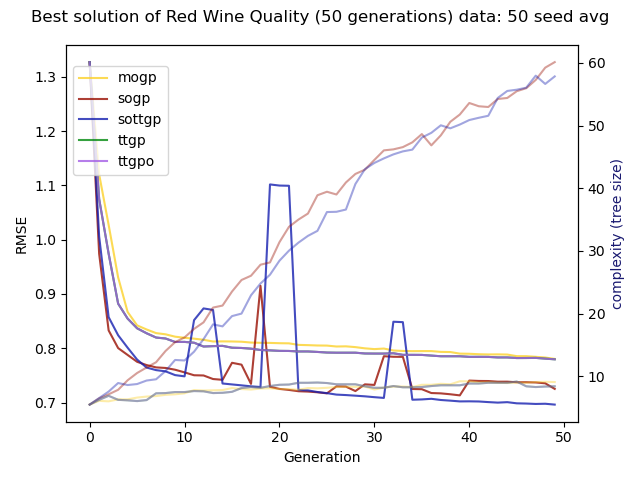
\includegraphics[width=0.40\textwidth]{Red Wine Quality (50 generations)-best-evo}
	\caption{Red Wine Quality (g250 p200) Testing}
	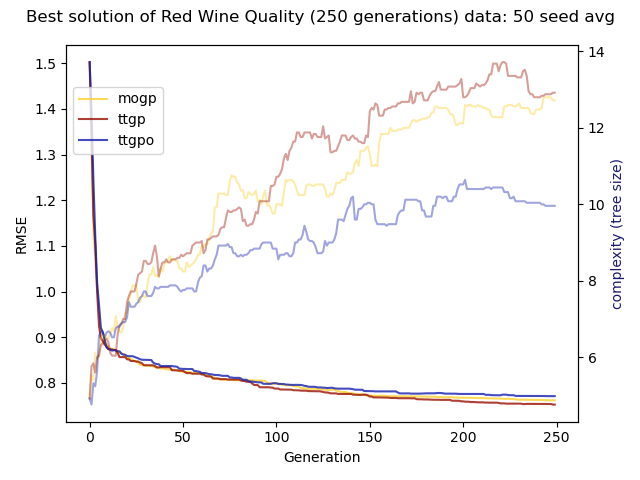
\includegraphics[width=0.40\textwidth]{Red Wine Quality (250 generations)-best-evo}
	\caption{White Wine Quality (g50 p500) Testing}
	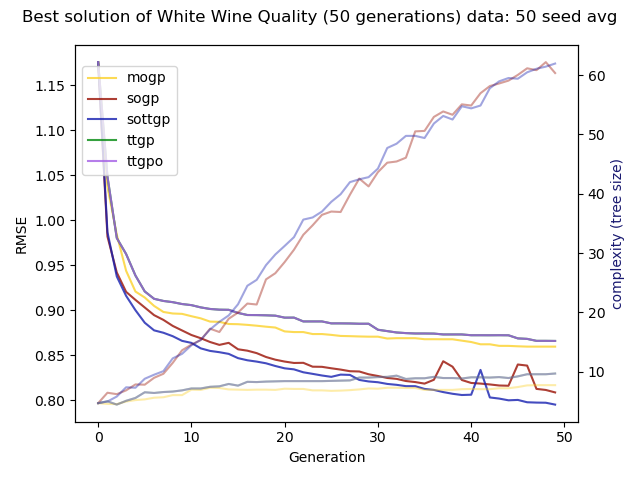
\includegraphics[width=0.40\textwidth]{White Wine Quality (50 generations)-best-evo}
	\caption{White Wine Quality (g250 p200) Testing}
	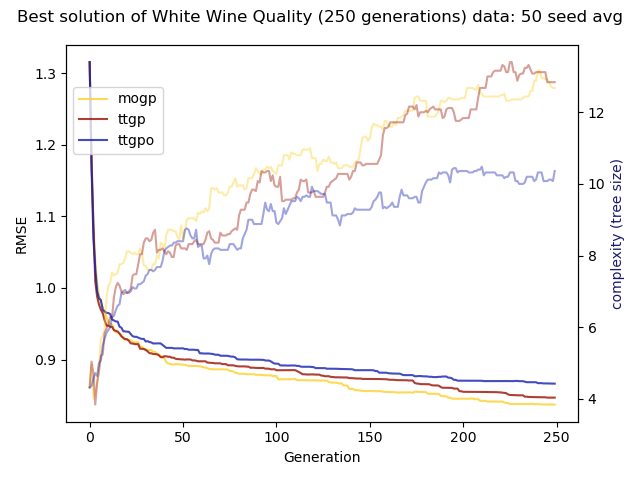
\includegraphics[width=0.40\textwidth]{White Wine Quality (250 generations)-best-evo}
\end{figure}
\begin{figure}[!htb]
	\caption{Red Wine Quality (g50 p500) Training}
	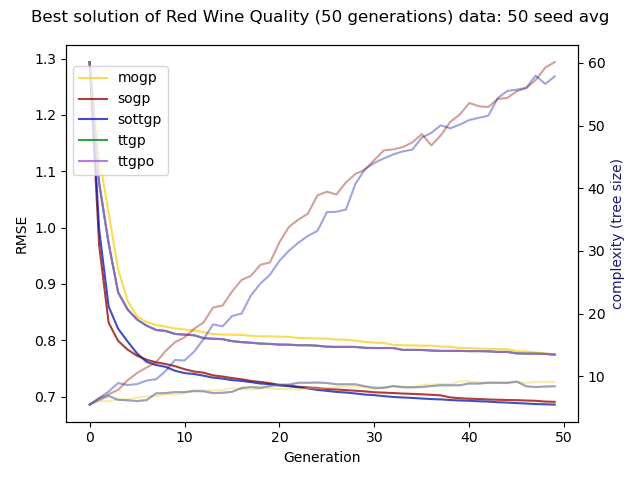
\includegraphics[width=0.40\textwidth]{Red Wine Quality (50 generations)-besttrain-evo}
	\caption{Red Wine Quality (g250 p200) Training}
	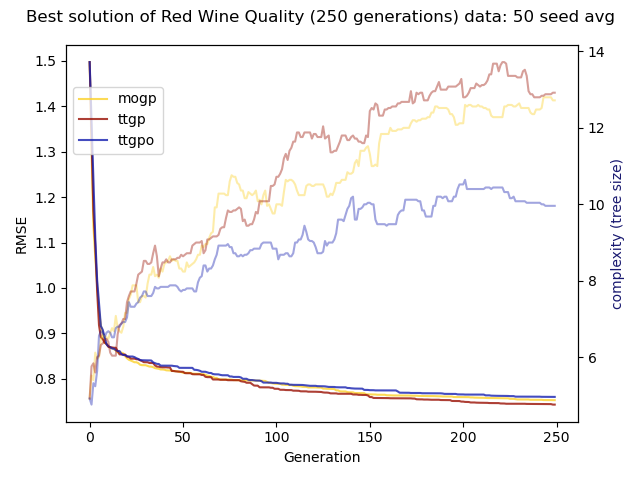
\includegraphics[width=0.40\textwidth]{Red Wine Quality (250 generations)-besttrain-evo}
	\caption{White Wine Quality (g50 p500) Training}
	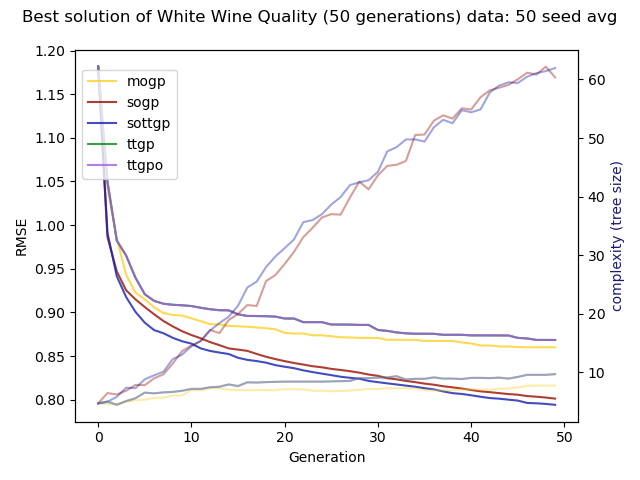
\includegraphics[width=0.40\textwidth]{White Wine Quality (50 generations)-besttrain-evo}
	\caption{White Wine Quality (g250 p200) Training}
	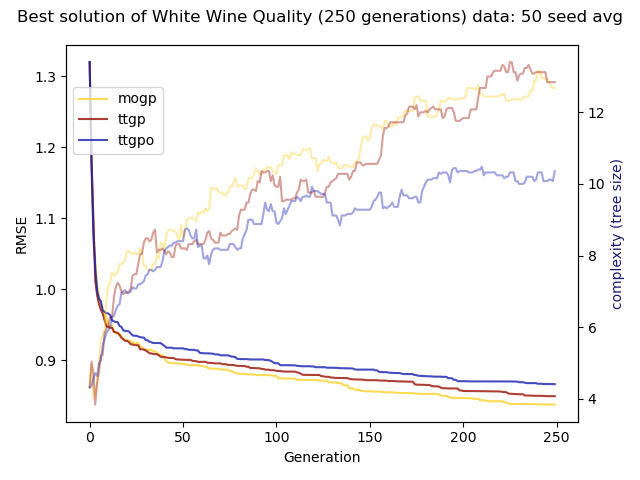
\includegraphics[width=0.40\textwidth]{White Wine Quality (250 generations)-besttrain-evo}
\end{figure}
\begin{figure}[!htb]
	\caption{Concrete Strength (g50 p500) Testing}
	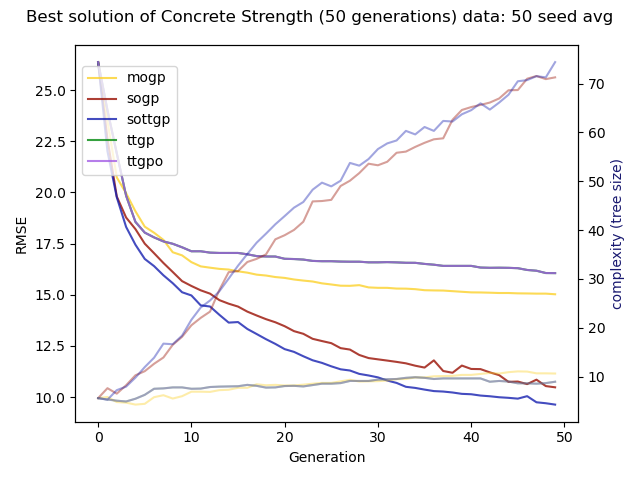
\includegraphics[width=0.40\textwidth]{Concrete Strength (50 generations)-best-evo}
	\caption{Concrete Strength (g250 p200) Testing}
	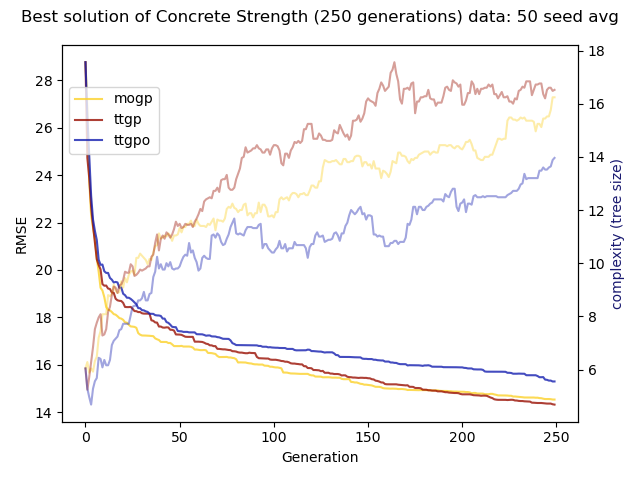
\includegraphics[width=0.40\textwidth]{Concrete Strength (250 generations)-best-evo}
	\caption{Boston House Price (g50 p500) Testing}
	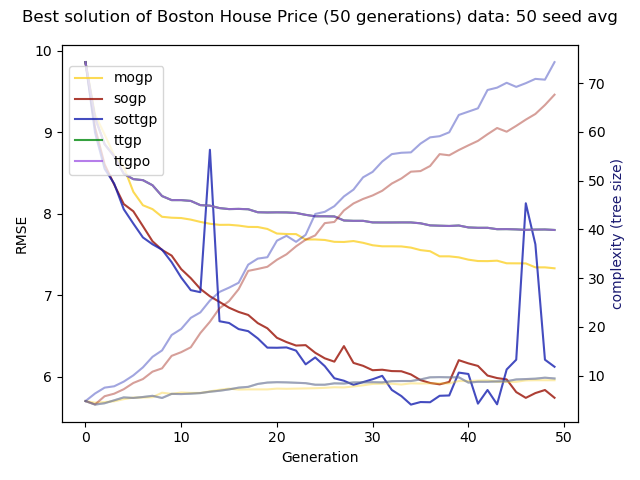
\includegraphics[width=0.40\textwidth]{Boston House Price (50 generations)-best-evo}
	\caption{Boston House Price (g250 p200) Testing}
	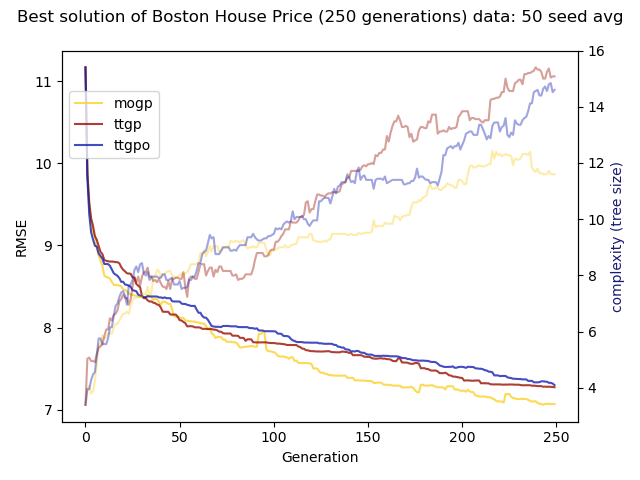
\includegraphics[width=0.40\textwidth]{Boston House Price (250 generations)-best-evo}
\end{figure}
\begin{figure}[!htb]
	\caption{Concrete Strength (g50 p500) Training}
	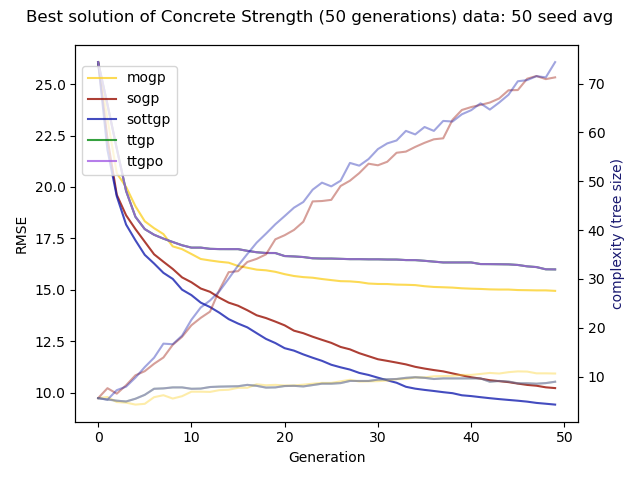
\includegraphics[width=0.40\textwidth]{Concrete Strength (50 generations)-besttrain-evo}
	\caption{Concrete Strength (g250 p200) Training}
	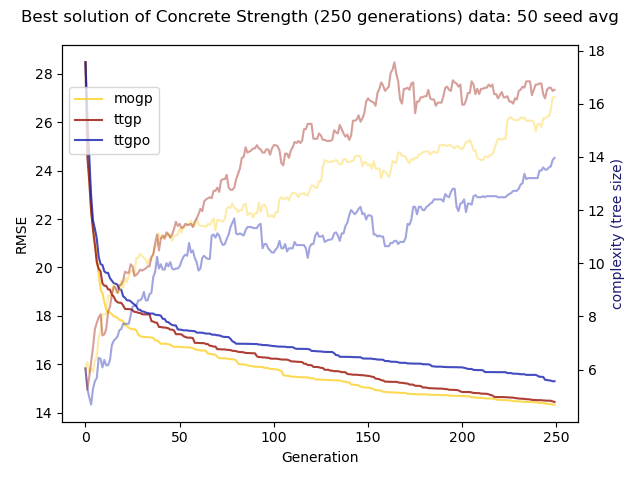
\includegraphics[width=0.40\textwidth]{Concrete Strength (250 generations)-besttrain-evo}
	\caption{Boston House Price (g50 p500) Training}
	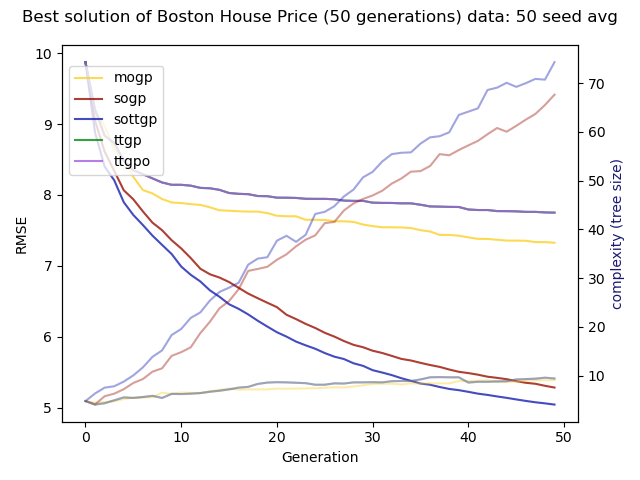
\includegraphics[width=0.40\textwidth]{Boston House Price (50 generations)-besttrain-evo}
	\caption{Boston House Price (g250 p200) Training}
	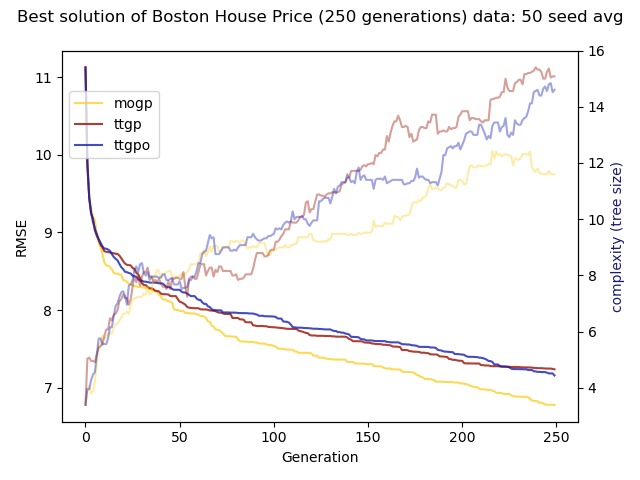
\includegraphics[width=0.40\textwidth]{Boston House Price (250 generations)-besttrain-evo}
\end{figure}
\end{document}